\normaltrue \difficilefalse \tdifficilefalse
\correctionfalse

%\UPSTIidClasse{11} % 11 sup, 12 spé
%\newcommand{\UPSTIidClasse}{12}

\exer{Calcul de moment$\star$ \label{B2:14-gl:520}}
\setcounter{numques}{0}
\UPSTIcompetence[2]{B2-14}
\index{Compétence B2-14}
%\index{La Seine Musicale}
\ifcorrection
\else
\textbf{Pas de corrigé pour cet exercice.}
\fi

\ifprof
\else


\begin{figure}[H]
\centering
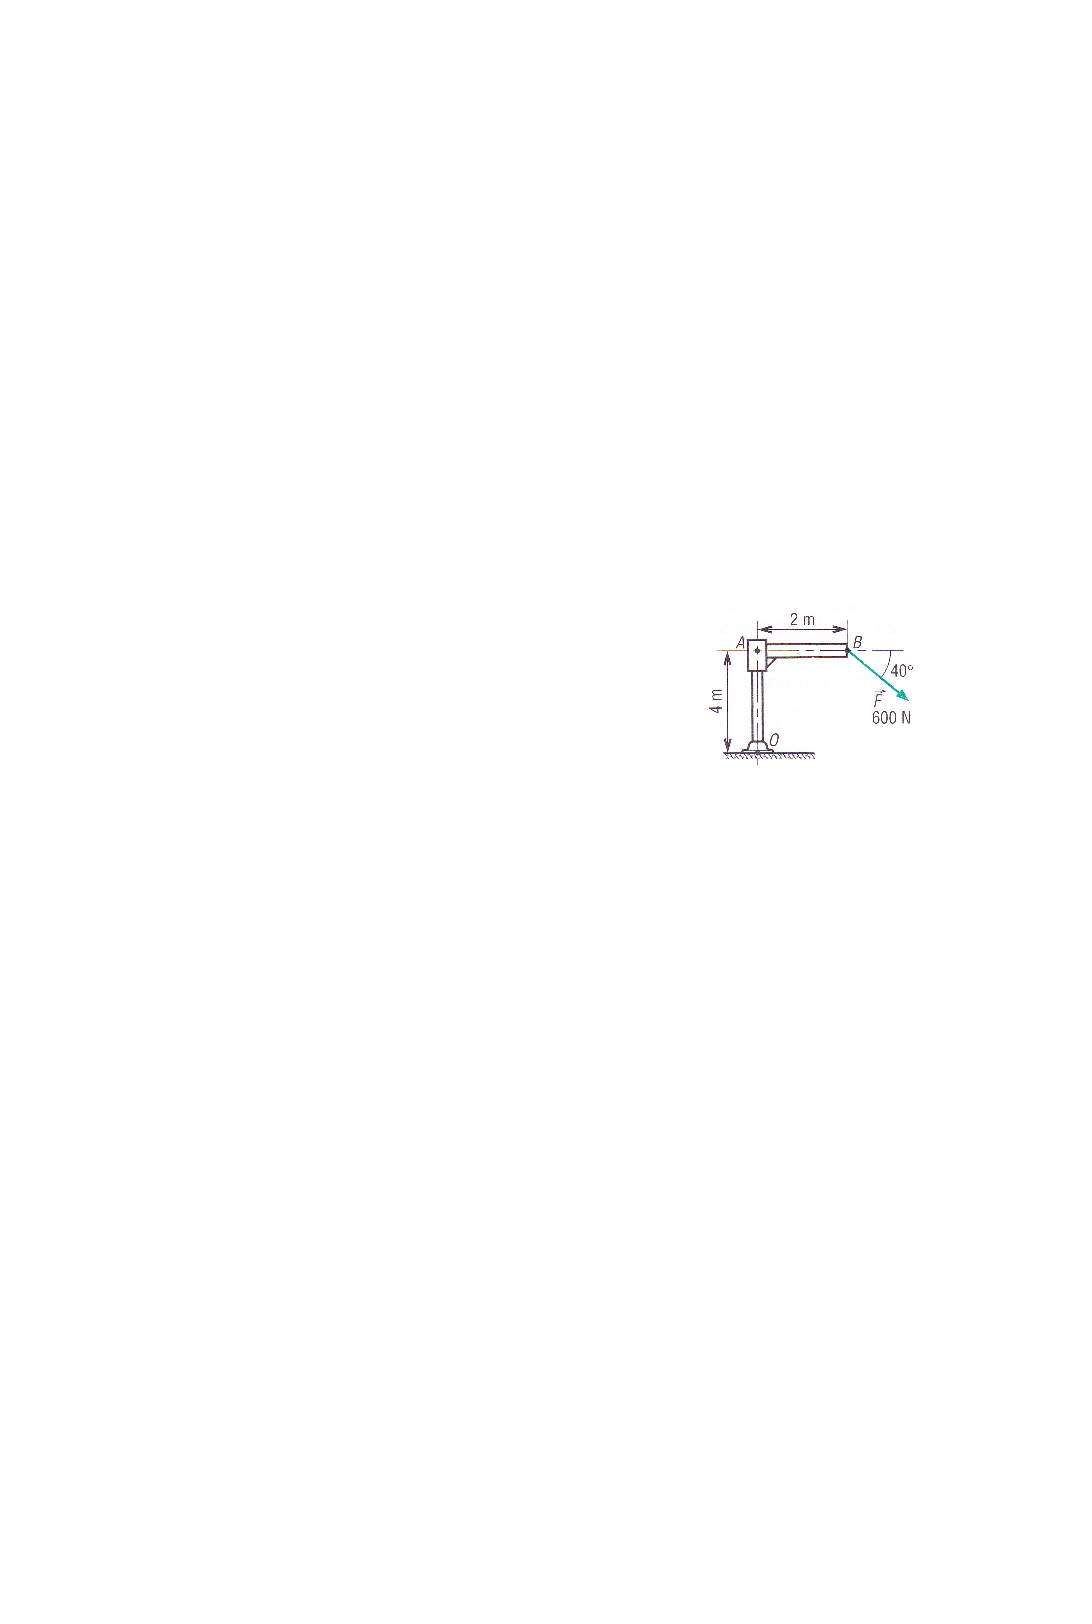
\includegraphics[width=\linewidth]{520_01}
%\caption{Paramétrage de la surface totale et élémentaire en coordonnées sphériques de la demi-voile \label{fig_39_01}}
\end{figure}


\question{Déterminer $\vect{\mathcal{M}\left(B,\vect{F}\right)}$.}%\vectm{A}{F}{1}{2}$.}
\ifprof ~\\
\else
\fi

\question{Déterminer $\vect{\mathcal{M}\left(O,\vect{F}\right)}$.}%\vectm{A}{F}{1}{2}$.}
\ifprof ~\\
\else
\fi


\ifprof
\else
\begin{flushright}
\footnotesize{Corrigé  voir \ref{B2:14-gl:520}.}
\end{flushright}%
\fi